\RequirePackage[l2tabu, orthodox]{nag}
\documentclass[ngerman, hyperref={pdfpagelabels=false}]{beamer}
%\documentclass[handout]{beamer}
\usepackage[ngerman]{babel}
\usepackage{amsmath}
\usepackage{amsfonts}
\usepackage{amssymb}
\usefonttheme{serif}
\usepackage[utf8]{inputenc}
\usepackage {graphicx}
\usepackage [T1]{fontenc}
%\usepackage{listings} %Quellcode mit \lstinline{} oder mit \begin ... darstellen
\usepackage{hyperref}
\usepackage{fancyvrb}

\usepackage{siunitx}
\usepackage{cancel}
\usepackage{slashed}
\usepackage{braket}

\usepackage{cprotect}

\usepackage{animate}
\usepackage{media9}
\usepackage{spreadtab}

%\usepackage{caption}
%\usepackage{subcaption}
%\captionsetup[subfigure]{labelformat=empty}

% TikZ
%\usepackage[landscape]{geometry}
%\usepackage{tikz}
%\usetikzlibrary{mindmap}
%\usepackage{metalogo}
%\usepackage{dtklogos}
%\usepackage{adjustbox}

\usepackage{bbding}
\usepackage{overpic}

\usepackage{cleveref}
%\crefname{equation}{Glg.}{Glgn.}

%\pgfpagesuselayout{4 on 1 with notes}[a4paper,border shrink=5mm]
\title[\LaTeX-Einführung]{Ausgewählite praktische Packages}
\institute{Fachschaft Physik}
\author[Ole, Marco]{Ole Hinrichs, Marco Knipfer}
%\usetheme{Warsaw}
\usetheme{Madrid}
\usecolortheme{default}
\beamertemplatenavigationsymbolsempty
\providecommand{\thispdfpagelabel}[1]{}

\begin{document} 


\begin{frame}[fragile]{Code in \LaTeX{} anzeigen lassen}{verbatim und das fancyvrb Package}
    \begin{block}{verbatim}
        \begin{itemize}
            \item entweder \verb+\verb!CODE!+
            \item oder \verb!\begin{verbatim} CODE \end{verbatim}!
                \pause
            \item Bei \textit{Beamer}
                \verb!\begin{frame}[fragile]{frametitle}! nötig
            \item empfehlenswert ist das \verb!\usepackage{fancyvrb}! Package
            \item 
            \begin{small}
                \begin{verbatim}
\begin{Verbatim}[frame=single, fontsize=\small, 
label={[Beginning of code]End of code}]
                \end{verbatim}
            \end{small}
        \end{itemize}
    \end{block}
    ~\\
    \begin{Verbatim}[frame=single, fontsize=\small, 
        label={[Beginning of code]End of code}]
code
code
    \end{Verbatim}
\pause
Auch Zeilennummerierung mit \verb!numers=left! (oder \verb!right!) mögllich.
\end{frame}
\begin{frame}[fragile]{Das Geometry Package}{Deutsche Anleitung
    \url{ftp://ftp.dante.de/pub/tex/macros/latex/contrib/geometry-de/geometry-de.pdf}}
\begin{minipage}{.49\textwidth}
    \begin{Verbatim}[frame=single] 
\usepackage{geometry}
\geometry{
    a4paper,
    total={170mm,257mm},
    left=20mm,
    top=20mm,
}
    \end{Verbatim}
\end{minipage}
    \pause
\begin{minipage}{.49\textwidth}
    \begin{tabular}{ll}
        left      & linke Randbreite \\
        righ      & rechte Randbreite \\
        width     & Breite \\
        heigt     & Höhe \\
        textwidth &Textreite \\
        textheight&Texthöhe \\
        top       &oberer Rand \\
        bottom    &unterer Rand \\
    \end{tabular}

\end{minipage}

\end{frame}
\begin{frame}[fragile]{Spreadtab}{Und es geht doch Tabellenkalkulation in \LaTeX{}}
    \verb!\usepackage{spreadtab}! \\
    \begin{minipage}{.39\textwidth}
        \begin{spreadtab}{{tabular}{rr|r}} 22 & 54 & a1+b1 \\
            43 & 65 & a2+b2 \\ 49 & 37 & a3+b3 \\
            \hline
            a1+a2+a3 & b1+b2+b3 & a4+b4
        \end{spreadtab}
    \end{minipage}
    \begin{minipage}{.6\textwidth}
        \begin{Verbatim}[frame=single]
\begin{spreadtab}{{tabular}{rr|r}} 
    22 & 54 & a1+b1 \\
    43 & 65 & a2+b2 \\ 
    49 & 37 & a3+b3 \\
    \hline
    a1+a2+a3 & b1+b2+b3 & a4+b4
\end{spreadtab}
        \end{Verbatim}
    \end{minipage}
    \pause
    \\ 
    ~\\~\\
    Wenn es euch interessiert: Lest die Anleitung dazu :P
    \\
    \url{ftp://ftp.tu-chemnitz.de/pub/tex/macros/latex/contrib/spreadtab/spreadtab_doc_en.pdf}
\end{frame}
\begin{frame}[fragile]{Die Optionen \textit{draft} und \textit{final} bei der
    \textit{documentclass}}
    \begin{block}{draft}
        \begin{itemize}
            \item \verb!\documentclass[draft]{scrartcl}!
            \item Kästen statt Bilder (graphicx)
            \item Keine Links (hyperref)
            \item Over-/underfull boxes werden am Rand angezeigt
            \item Viel schneller!
        \end{itemize}
    \end{block}
    \pause
    \begin{block}{final}
        \begin{itemize}
            \item \verb!\documentclass[final]{beamer}!
            \item Default für die meisten Klassen
                \pause
            \item Zum Beispiel Todonotes:\\
                \verb!\usepackage[obeyfinal]{todonotes}!\\
            \item[$\rightarrow$] Keine Todonotes falls final
        \end{itemize}
    \end{block}
\end{frame}
\begin{frame}[fragile]{Für Interessierte -- Das \LaTeXe{}-Sündenregister}
    {oder Veraltete Befehle, Pakete und andere Fehler \\
    \url{ftp://ftp.dante.de/tex-archive/info/l2tabu/german/l2tabu.pdf}
}
    \begin{block}{Beispiele}
        \begin{itemize}
            \item nicht \verb!$$ formel $$! für abgesetzte Formeln
                werwenden, da \TeX{} Befehl.
            \item[$\rightarrow$] Vertikalen Abstäde bei abgesetzten Formeln
                werden inkonsistent.
            \item \verb!\centering! statt \verb!\begin{center}! in
                    float-Umgebungen
            \item \dots
        \end{itemize}
    \end{block}
    \pause
    \centering
    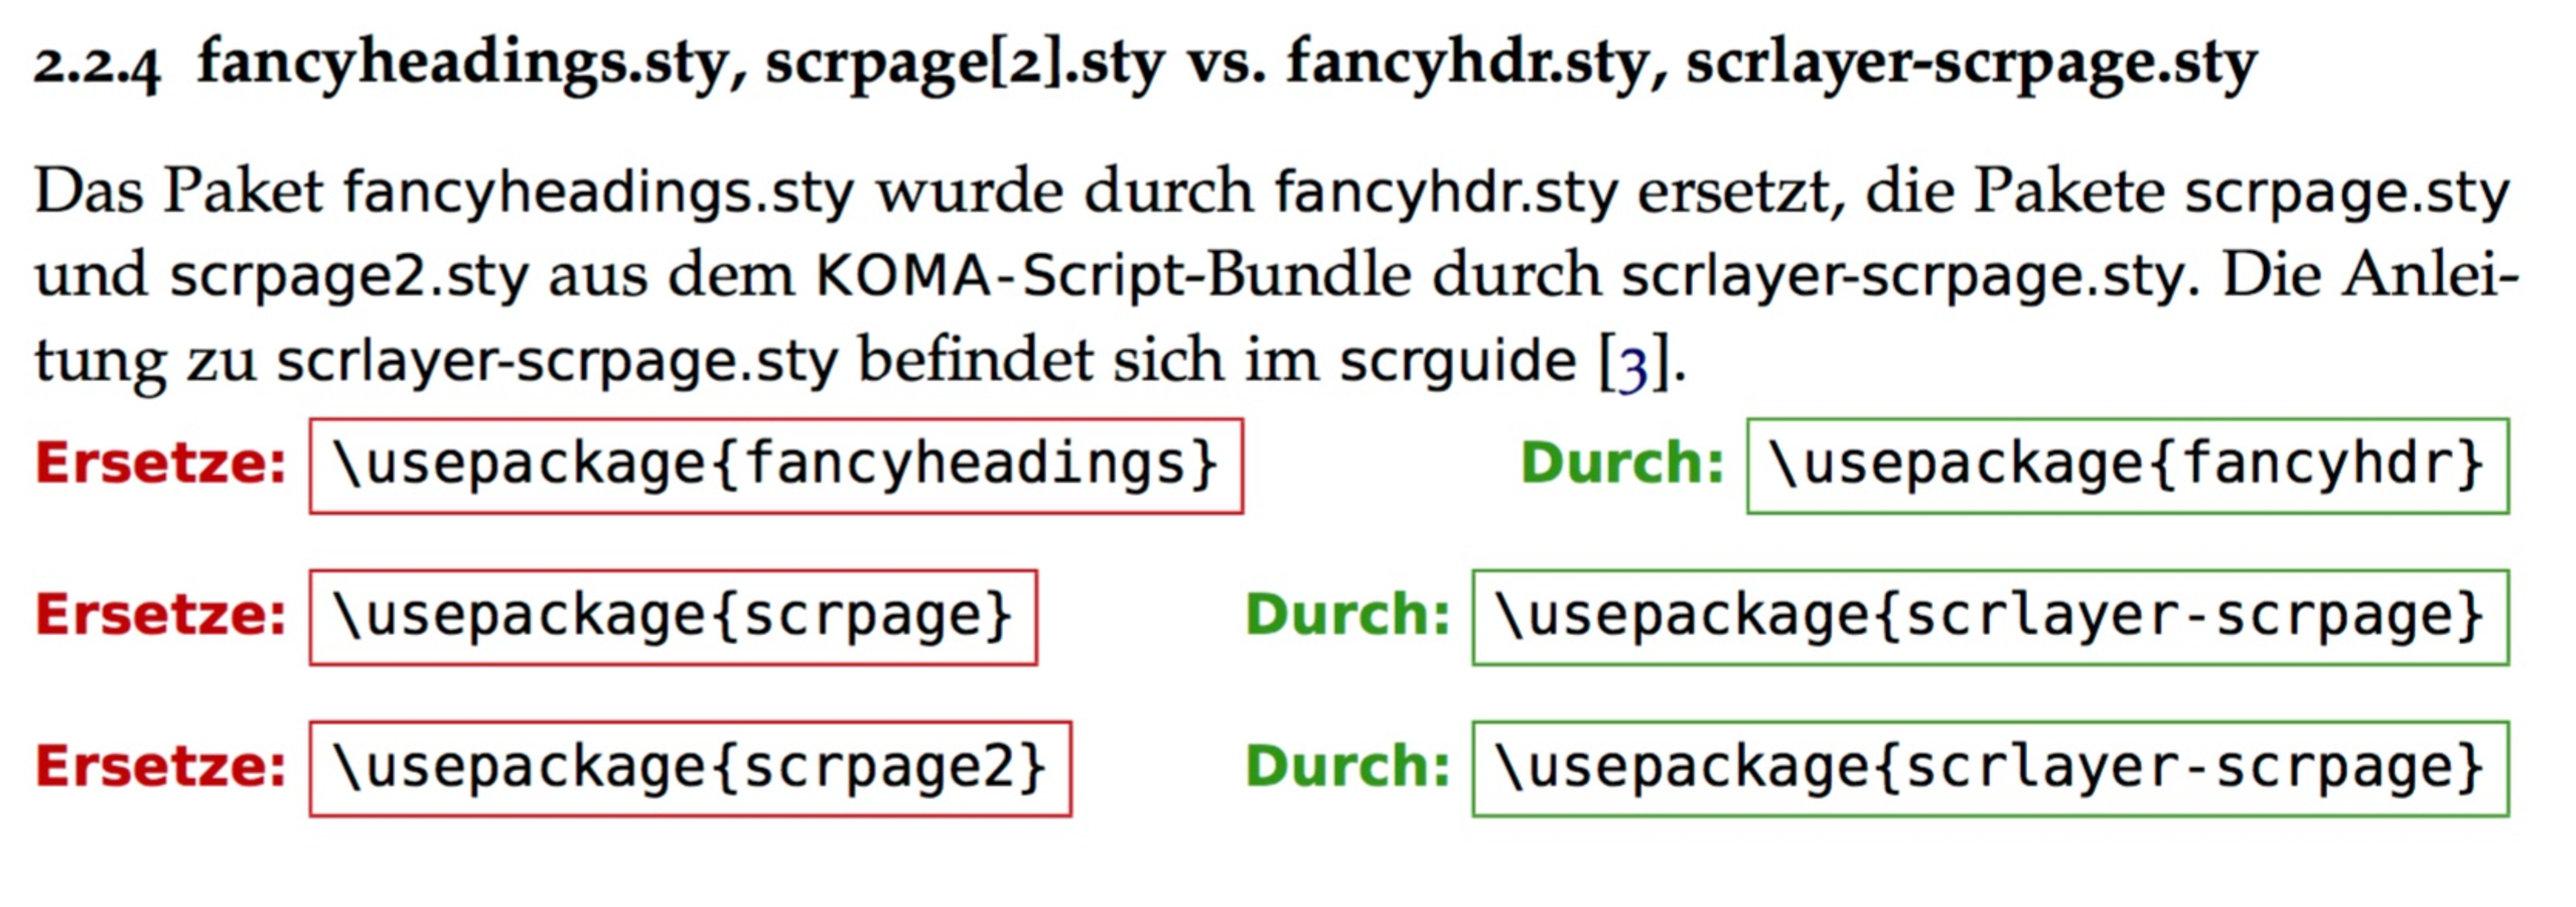
\includegraphics[width=0.9\textwidth]{figures/suenden.pdf}
\end{frame}
\begin{frame}[fragile]{Das \textit{nag} Package}
    {Im .log File Hinweise auf deprecated Packages oder Befehle}
    \begin{Verbatim}
\RequirePackage[l2tabu, orthodox]{nag}
\documentclass{scrartcl}
.
.
.
    \end{Verbatim}
\end{frame}

\begin{frame}[fragile]{Das \textit{cleverref} Package}{Einfachere ref-Befehle}
    \begin{block}{}
        \begin{itemize}
            \item Standard: \verb!Gleichung~(\ref{eq:eq1})!
            \item Später willst du dann \verb!Glg.~(\ref{eq:eq1})!
                \pause
            \item \verb!\usepackage{cleveref}!
            \item statt \verb!\ref{}! jetzt \verb!\cref{}!
            \item \verb!\cref{eq1}! statt \verb!Gleichung~(\ref{eq1})!
        \end{itemize}
    \end{block}
\end{frame}
\begin{frame}[fragile]{Beispiel cref}
    \begin{equation}
        a^2 + b^2 = c^2
        \label{eq:pythagoras}
    \end{equation}
    \cprotect\fbox{
        \begin{minipage}{.85\textwidth}
        ref:\\
        Wie in Gleichung~(\ref{eq:pythagoras}) zu sehen ist
        \begin{Verbatim}
Wie in Gleichung~(\ref{eq:pythagoras}) zu sehen ist
        \end{Verbatim}
    \end{minipage}
}
\\ ~\\~\\
    \cprotect\fbox{
        \begin{minipage}{.85\textwidth}
        cref:\\
        Wie in \cref{eq:pythagoras} zu sehen ist
        \begin{Verbatim}
Wie in \cref{eq:pythagoras} zu sehen ist
        \end{Verbatim}
    \end{minipage}
}
    \pause
    \\
    \bigskip
    Anpassung mit z.B.\ \verb!\crefname{equation}{Glg.}{Glgn.}!
\end{frame}

\end{document}
